\documentclass[a4paper,10pt]{report}\input{../0.Préambule/Préambule_cours_prof}\begin{document}

\pagestyle{empty}
\newpage
\section*{Les nombres relatifs \hspace{3cm} Sujet A}
\addcontentsline{toc}{section}{Produits de nombres relatifs}

\noindent \textit{L'usage de la calculatrice est \textbf{interdite}.} \hfill \textit{Durée : 30 minutes}

\paragraph{Exercice 1} : \hfill \textbf{3 points}

Complète avec le mot qui convient : 
 \og positif \fg{} \quad \og négatif \fg{} \quad \og plus \fg{} \quad \og relatifs \fg{} \quad \og opposé \fg{} \quad\og moins \fg{}

\begin{enumerate}
\item $-3$; $+5$; $-9,3$; $100,7$ et $0$ sont des nombres \dotfill \medskip
%\item Le nombres $+5$ est un nombre \dotfill \medskip
%\item Il peut aussi s'écrire sans le signe \dotfill \medskip
\item Le nombre $-5$ est un nombre \dotfill \medskip
\item On ne peut pas supprimer le signe \dotfill \medskip
%\item $-2,7$ est  \dotfill de $+2,7$.
\end{enumerate}

\paragraph{Exercice 2} : \hfill \textbf{9 points}

\begin{enumerate}
\item Sur la droite gradué ci dessous, place les points $A(+8)$, $B(-2)$, $C(+3)$, $D(-5)$ et $E(+2)$.

\begin{center}
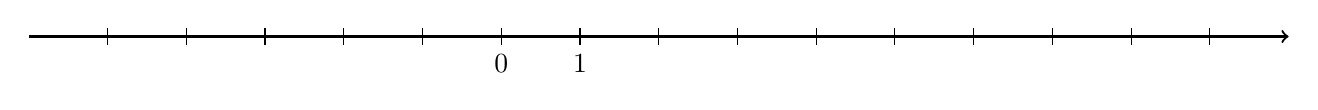
\begin{tikzpicture}[x=1cm]  
\draw[thick,->] (-6,0) -- (10,0);
\foreach \x in {0,1}
\draw[shift={(\x,0)},color=black] (0pt,3pt) -- (0pt,-3pt) node [below] {\x};
\foreach \x in {-5,-4,-3,-2,-1,2,3,4,5,6,7,8,9}	
\draw[shift={(\x,0)},color=black] (0pt,3pt) -- (0pt,-3pt) ;
\end{tikzpicture}
\end{center}

\vspace{-5mm}
\item En examinant la position des points $A$, $B$, $C$, $D$ et $E$ sur cette droite gradué, complète par $<$ou $>$ :
\begin{enumerate}
\renewcommand{\arraystretch}{1}
\begin{tabularx}{\linewidth}{*{5}{>{\arraybackslash}X}}
\item $2 ~\dots ~ \dots ~ -2$&
\item $+2 ~\dots ~ \dots ~ -5$&
%\item $+3 ~\dots ~ \dots ~ +8$&
\item $-2 ~\dots ~ \dots ~ -5$&
\item $+8 ~\dots ~ \dots ~ -2$&
\item $-5 ~\dots ~ \dots ~ +3$\\
\end{tabularx}
\end{enumerate}
\item Range dans l'ordre croissant : $+8$, $-2$, $+3$, $-5$ et $+2$.

\medskip \dotfill 
\end{enumerate}

\paragraph{Exercice 3} : \hfill \textbf{8 points}

Complète par $<$, $>$ ou $=$
\begin{enumerate}
\renewcommand{\arraystretch}{1}
\begin{tabularx}{\linewidth}{*{4}{>{\arraybackslash}X}}
%\item $10 ~\dots ~ \dots ~ +3$&
%\item $-5 ~\dots ~ \dots ~ -5,0$&
\item $-8 ~\dots ~ \dots ~ 0$&
%\item $0 ~\dots ~ \dots ~ -4$&
\item $+3 ~\dots ~ \dots ~ 0$&
%\item $-7 ~\dots ~ \dots ~ -8$&
\item $+250 ~\dots ~ \dots ~ +205$&
%\item $-82 ~\dots ~ \dots ~ -83$&
\item $-205 ~\dots ~ \dots ~ -2050$\\
%\item $+5,34 ~\dots ~ \dots ~ +3,54$&
\item $0,05 ~\dots ~ \dots ~ 1$&
%\item $-8,51 ~\dots ~ \dots ~ -8,5$&
\item $11,9 ~\dots ~ \dots ~ +11,9$&
%\item $3,14 ~\dots ~ \dots ~ -1,732$&
\item $-9,27 ~\dots ~ \dots ~ -9,272$&
%\item $+8,64 ~\dots ~ \dots ~ -8,64$&
%\item $-19,2 ~\dots ~ \dots ~ +9,2$&
\item $-14,39 ~\dots ~ \dots ~ +14,4$\\
\end{tabularx}
\end{enumerate}

\section*{Les nombres relatifs \hspace{3cm} Sujet B}
\addcontentsline{toc}{section}{Produits de nombres relatifs}

\noindent \textit{L'usage de la calculatrice est \textbf{interdite}.} \hfill \textit{Durée : 30 minutes}

\paragraph{Exercice 1} : \hfill \textbf{3 points}

Complète avec le mot qui convient : 
 \og positif \fg{} \quad \og négatif \fg{} \quad \og plus \fg{} \quad \og relatifs \fg{} \quad \og opposé \fg{} \quad\og moins \fg{}

\begin{enumerate}
%\item $-3$; $+5$; $-9,3$; $100,7$ et $0$ sont des nombres \dotfill \medskip
\item Le nombres $+5$ est un nombre \dotfill \medskip
\item Il peut aussi s'écrire sans le signe \dotfill \medskip
%\item Le nombre $-5$ est un nombre \dotfill \medskip
%\item On ne peut pas supprimer le signe \dotfill \medskip
\item $-2,7$ est  \dotfill de $+2,7$.
\end{enumerate}

\paragraph{Exercice 2} : \hfill \textbf{9 points}

\begin{enumerate}
\item Sur la droite gradué ci dessous, place les points $A(-4)$, $B(+2)$, $C(+4)$, $D(-3)$ et $E(-2)$.

\begin{center}
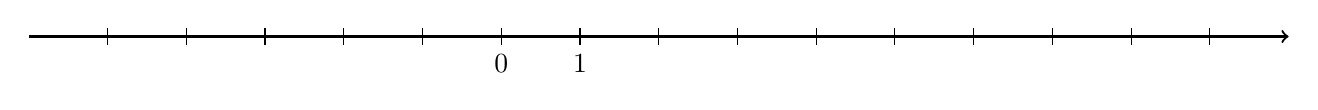
\begin{tikzpicture}[x=1cm]  
\draw[thick,->] (-6,0) -- (10,0);
\foreach \x in {0,1}
\draw[shift={(\x,0)},color=black] (0pt,3pt) -- (0pt,-3pt) node [below] {\x};
\foreach \x in {-5,-4,-3,-2,-1,2,3,4,5,6,7,8,9}	
\draw[shift={(\x,0)},color=black] (0pt,3pt) -- (0pt,-3pt) ;
\end{tikzpicture}
\end{center}

\vspace{-5mm}
\item En examinant la position des points $A$, $B$, $C$, $D$ et $E$ sur cette droite gradué, complète par $<$ou $>$ :
\begin{enumerate}
\renewcommand{\arraystretch}{1}
\begin{tabularx}{\linewidth}{*{5}{>{\arraybackslash}X}}
\item $2 ~\dots ~ \dots ~ -2$&
\item $+2 ~\dots ~ \dots ~ -3$&
%\item $+3 ~\dots ~ \dots ~ +8$&
\item $-2 ~\dots ~ \dots ~ -3$&
\item $-4 ~\dots ~ \dots ~ -2$&
\item $-3 ~\dots ~ \dots ~ +3$\\
\end{tabularx}
\end{enumerate}
\item Range dans l'ordre croissant : $-4$, $+2$, $+3$, $-3$ et $-2$.

\medskip \dotfill 
\end{enumerate}

\paragraph{Exercice 3} : \hfill \textbf{8 points}

Complète par $<$, $>$ ou $=$
\begin{enumerate}
\renewcommand{\arraystretch}{1}
\begin{tabularx}{\linewidth}{*{4}{>{\arraybackslash}X}}
\item $10 ~\dots ~ \dots ~ +3$&
%\item $-5 ~\dots ~ \dots ~ -5,0$&
%\item $-8 ~\dots ~ \dots ~ 0$&
\item $0 ~\dots ~ \dots ~ -4$&
%\item $+3 ~\dots ~ \dots ~ 0$&
\item $-7 ~\dots ~ \dots ~ -8$&
%\item $+250 ~\dots ~ \dots ~ +205$&
\item $-82 ~\dots ~ \dots ~ -83$\\
%\item $-205 ~\dots ~ \dots ~ -2050$\\
\item $+5,34 ~\dots ~ \dots ~ +3,54$&
%\item $0,05 ~\dots ~ \dots ~ 1$&
\item $-8,51 ~\dots ~ \dots ~ -8,5$&
%\item $11,9 ~\dots ~ \dots ~ +11,9$&
\item $3,14 ~\dots ~ \dots ~ -1,732$&
%\item $-9,27 ~\dots ~ \dots ~ -9,272$&
\item $+8,64 ~\dots ~ \dots ~ -8,64$\\
%\item $-19,2 ~\dots ~ \dots ~ +9,2$&
%\item $-14,39 ~\dots ~ \dots ~ +14,4$\\
\end{tabularx}
\end{enumerate}
\end{document}
